\newchapter{c:commissioning}{Commissioning of the PFF System}

This is the introductory text.

\newsection{s:daq}{Controls}

\newsection{s:droopCorr}{Droop Correction}

The droop in the response of the FONT5 ADCs, as most clearly seen in the output of the diode channel in Figure \ref{f:diodeDroop} (although it also effects the mixer channel), is not an issue for the work the FONT group does at ATF2 where the signals are well approximated by delta functions separated by \(\sim\)100~ns. Although the droop has been seen previously, its significance for the continuous microsecond length pulse at CTF3 had not been considered because of this.

\begin{figure}
  \centering
  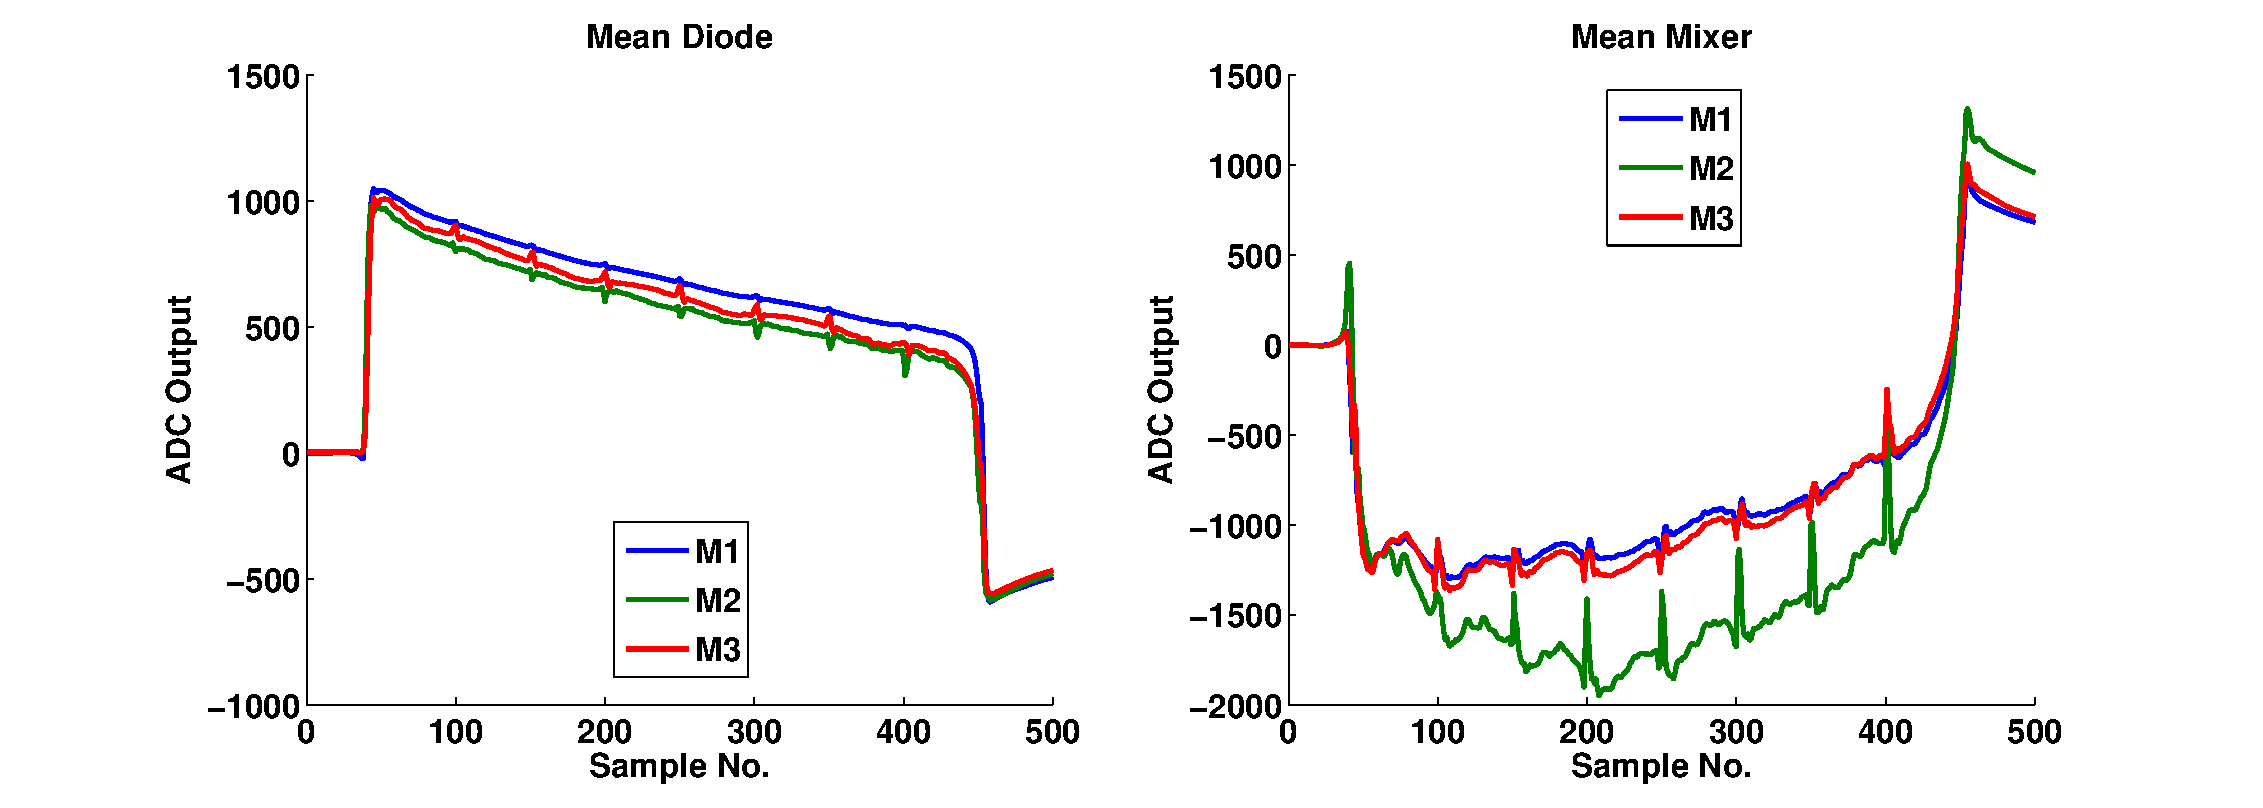
\includegraphics[width=0.9\textwidth]{Figures/diodeDroop}
  \caption{Mean diode and mixer output with no filter.}
  \label{f:diodeDroop}
\end{figure}

The droop emerges as a result of the use of AC coupling on the ADC input transformers for electrical isolation. This involves using a capacitor, the current across which is dependent on \({dV}/{dt}\) (\(V\) being voltage and \(t\) time), to remove the DC component from a signal. In particular for the diode channel, which should be a square wave, the output is increasingly well described by a DC signal on the flat top as you move away from the leading edge of the pulse, with the capacitor causing droop in the response as a result.

In the simplest case the droop should be well described by an exponential decay of the form \(A\exp\left(-t/T\right)\). The droop makes it difficult to perform calibrations and measurements on the data and one way in which it could be removed in offline analysis is by determining the decay constants, \(T\), for each of the ADCs on the FONT5 board. To avoid the influence of beam effects tests were done in Oxford using a generated 10~\(\mu\)s DC pulse.

\begin{figure}
  \centering
  \includegraphics[width=0.45\textwidth]{Figures/droopFit}
  \caption{Attempted exponential fit to the ADC droop.}
  \label{f:droopFit}
\end{figure}

Unfortunately, as can be seen in Figure \ref{f:droopFit} which shows an example of an exponential fit for one ADC, although the fits return good \(R^{2}\) values it is clear that the slope of the exponential curve is not a good match for the slope of the data. This is perhaps not unexpected as the ferrite cores used in the transformers have many non-linear properties. In fact, by using a fit with two exponential terms it is possible to obtain a perfect match to the data but at this point the complexity of the fit would make any attempt to remove the droop in real beam data in this way spurious.

Instead, changes will be made to the currently in development FONT5a board hardware and firmware to greatly reduce the scale of the droop. Different transformers will be used to reduce the droop rate by up to a factor of fifty and in addition digital filtering will be implemented in firmware to smooth out and reduce the remaining droop component even further. It is expected that after these changes the droop will be small enough to not have a detrimental effect on the performance of the phase feedforward system. 

\newsection{s:constKicks}{Constant Kick Tests}

Scan and comparison to expectation from optics.

Linearity

Orbit closure

Shape of FF kick on BPMs vs. shape of upstream phase

\newsection{s:latency}{Latency Measurements}

\newsection{s:timing}{Kick Output Timing}

\subsection{Relative Kicker Timing}
\label{ss:relativeTiming}


\subsection{Absolute Kicker Timing}
\label{ss:relativeTiming}

from beam pickup

from kick on BPMs

\newsection{s:slowCorr}{Slow Correction}







